\documentclass[a4paper,14pt]{extarticle} 
\usepackage[a4paper,top=1.5cm, bottom=1.5cm, left=2cm, right=1cm]{geometry}
%\usepackage[T2A]{fontenc}
%\usepackage[english, russian]{babel}
\usepackage{graphicx}
\DeclareGraphicsExtensions{.pdf,.png,.jpg}

\usepackage{fontspec}
\setmainfont{Times New Roman}
\setsansfont{FreeSans}
\setmonofont{FreeMono}
\renewcommand{\baselinestretch}{1.5}
\usepackage{polyglossia}
\setdefaultlanguage{russian}
\setotherlanguages{english,russian}
\usepackage{setspace}
\usepackage[many]{tcolorbox}
\usepackage{listings}
\usepackage{xcolor}

\definecolor{codegreen}{rgb}{0,0.6,0}
\definecolor{codegray}{rgb}{0.5,0.5,0.5}
\definecolor{codepurple}{rgb}{0.58,0,0.82}
\definecolor{backcolour}{rgb}{0.95,0.95,0.92}

\lstdefinestyle{mystyle}{
    backgroundcolor=\color{backcolour},   
    keywordstyle=\color{magenta},
    numberstyle=\tiny\color{codegray},
    stringstyle=\color{codepurple},
    basicstyle=\ttfamily\footnotesize,
    breakatwhitespace=false,         
    breaklines=true,                 
    captionpos=b,                    
    keepspaces=true,                 
    numbers=left,                    
    numbersep=5pt,                  
    showspaces=false,                
    showstringspaces=false,
    showtabs=false,                  
    tabsize=2
}

\lstset{style=mystyle}

\begin{document}
    \begin{center}
        \thispagestyle{empty}
        \begin{singlespace}
        ФЕДЕРАЛЬНОЕ АГЕНТСТВО СВЯЗИ

        ФЕДЕРАЛЬНОЕ ГОСУДАРСТВЕННОЕ БЮДЖЕТНОЕ ОБРАЗОВАТЕЛЬНОЕ

        УЧРЕЖДЕНИЕ ВЫСШЕГО ОБРАЗОВАНИЯ

        «САНКТ-ПЕТЕРБУРГСКИЙ ГОСУДАРСТВЕННЫЙ УНИВЕРСИТЕТ ТЕЛЕКОММУНИКАЦИЙ ИМ. ПРОФ. М.А. БОНЧ-БРУЕВИЧА»

        (СПбГУТ)
        \end{singlespace}
        \vspace{-1ex}
        \rule{\textwidth}{0.4pt}
        \vspace{-5ex}

        Факультет \underline{Инфокоммуникационных сетей и систем}

        Кафедра \underline{Защищенных систем связи}
        \vspace{10ex}

        \textbf{Лабораторная работа №4}\\
    Управление операционной системой Cisco IOS и конфигурационными файлами на базе коммутаторов
        


    \end{center}
    \vspace{4ex}
    \begin{flushright}
    \parbox{10 cm}{
    \begin{flushleft}
        Выполнили студенты группы ИКТЗ-83:

        \underline{Громов А.А., Миколаени М.С., Мазеин Д.С.} \hfill \rule[-0.85ex]{0.1\textwidth}{0.6pt}

        \footnotesize \textit{ (Ф.И.О., № группы) \hfill (подпись)} \normalsize

        Проверил:

        \underline{Скорых М.А.} \hfill \rule[-0.85ex]{0.1\textwidth}{0.6pt}

        (\footnotesize \textit{уч. степень, уч. звание, Ф.И.О.) \hfill (подпись)} \normalsize

    \end{flushleft}
    }
    \end{flushright}
    \begin{center}
        \vfill
        Санкт-Петербург

        2021

    \end{center}
    \newpage

    \begin{center}
        \textbf{Установка обновления Cisco IOS}
    \end{center}
    \begin{center}
        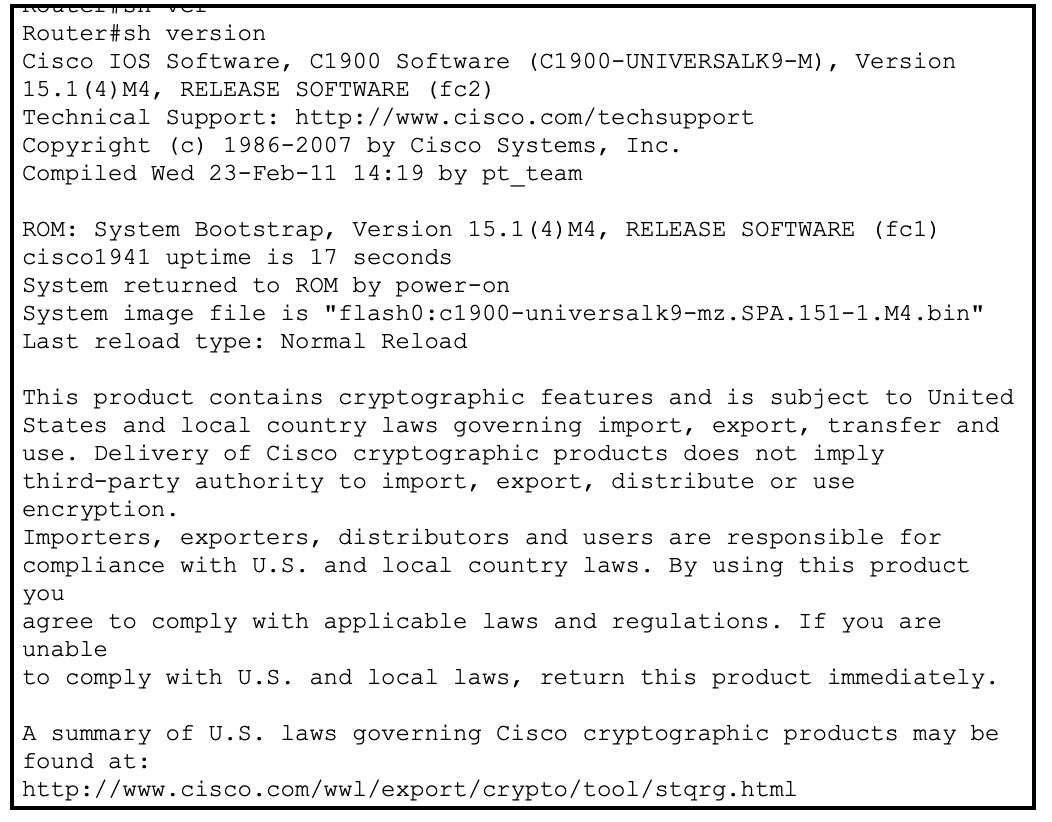
\includegraphics[scale=0.34]{pics/0.jpeg}
    \end{center}
    \begin{lstlisting}
copy tftp flash
10.0.0.2
c1900-universalk9-mz.SPA.155-3.M4a.bin
    \end{lstlisting}
    \begin{center}
        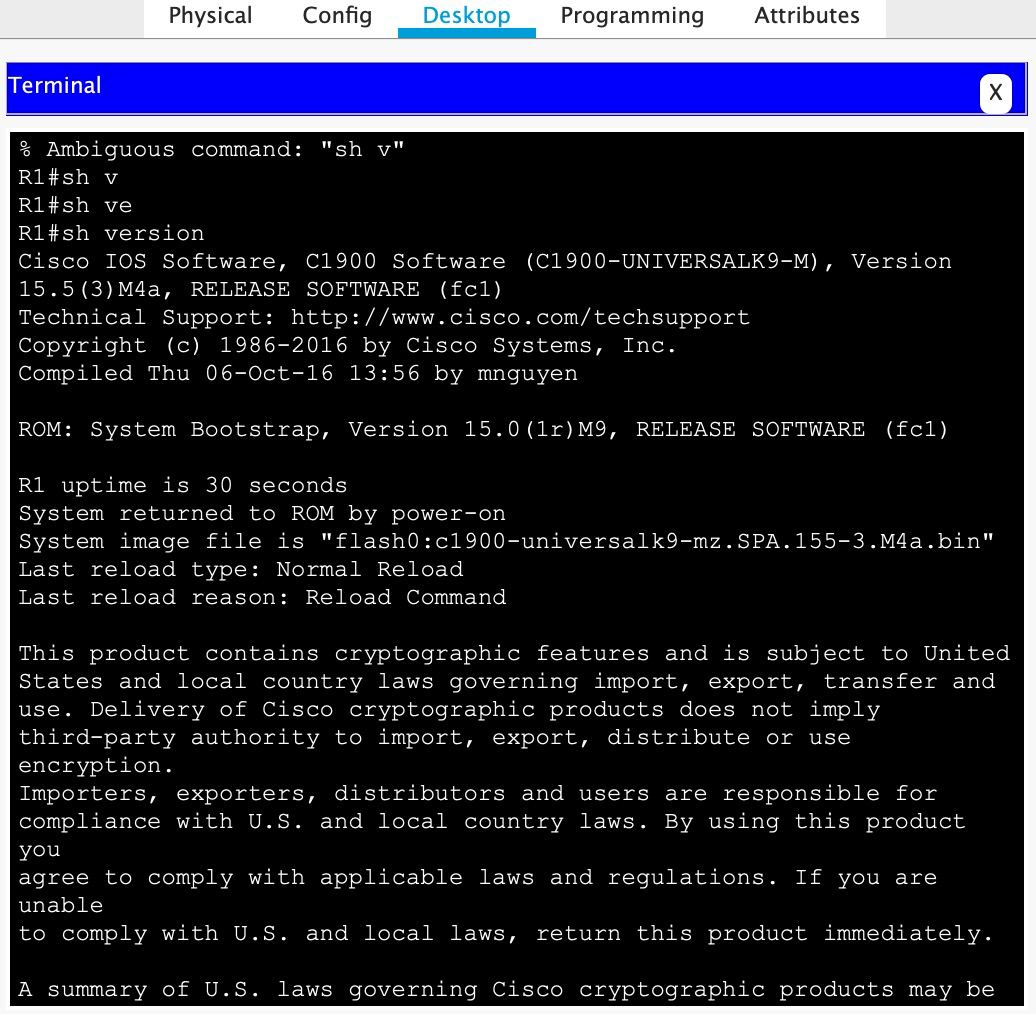
\includegraphics[scale=0.34]{pics/1.jpeg}
    \end{center}
    \begin{center}
        \textbf{Сброс пароля консольной линии}
    \end{center}
    При загрузке нажать control+C, затем:
    \begin{lstlisting}
confreg 0x2142.
    \end{lstlisting} 
    Система загрузится со стандартной конфигурацией. Далее, для того, чтобы восстановить предыдущую конфигурацию, нужно ввести команду:
    \begin{lstlisting}
copy startup-config running-config. 
    \end{lstlisting}    
    Теперь можно заменить забытый пароль, и сохранить новый пароль командой 
    \begin{lstlisting}
        copy running-config startup-config.
    \end{lstlisting}
\end{document}